\documentclass[a4paper,twocolumn]{oblivoir}
\usepackage{amsmath,amssymb,amsthm,kotex,graphicx,mdframed}
\usepackage{fapapersize}
\usefapapersize{210mm,297mm,10mm,*,10mm,*}
\newcounter{num}
\newcommand{\defi}[1]
{\bigskip\noindent\refstepcounter{num}\textbf{정의 \arabic{num}) #1}\par\noindent}
\newcommand{\theo}[1]
{\bigskip\noindent\refstepcounter{num}\textbf{정리 \arabic{num}) #1}\par\noindent}
\newcommand{\exam}[1]
{\bigskip\noindent\refstepcounter{num}\textbf{예시 \arabic{num}) #1}\par\noindent}
\newcommand{\prob}[1]
{\bigskip\noindent\refstepcounter{num}\textbf{문제 \arabic{num}) #1}\par\noindent}
\newcommand{\proo}
{\bigskip\textsf{증명)}\par}

\newcommand{\pb}[1]%\Phantom + fBox
{\fbox{\phantom{\ensuremath{#1}}}}

\title{수지 : 다항함수의 미분 복습}
\date{\today}
\author{}
%%%%
\begin{document}
\maketitle

%
\begin{mdframed}[frametitle=함수의 극한]
극한값 \(\displaystyle\lim_{x\to a}f(x)\)가 존재한다.\\
\(\displaystyle\iff\pb{\displaystyle\lim_{x\to a-}f(x)}=\pb{\displaystyle\lim_{x\to a+}f(x)}\)
\end{mdframed}

%
\begin{mdframed}[frametitle=함수의 연속]
\(f(x)\)가 \(x=a\)에서 연속이다.\\
\(\iff\pb{\displaystyle\lim_{x\to a}f(x)}=\pb{f(a)}\)
\end{mdframed}

%
\begin{mdframed}[frametitle=평균변화율]
\[f(x)\text{의 }x=a\text{에서 }x=b\text{까지의 평균변화율}=\frac{f(b)-f(a)}{b-a}\]
\end{mdframed}

%
\begin{mdframed}[frametitle=순간변화율(=미분계수)]
\begin{align*}
f(x)\text{의 }x=a\text{에서의 순간변화율}=&f'(a)\\
=&\lim_{x\to a}\frac{f(x)-f(a)}{x-a}\\
=&\lim_{h\to0}\frac{f(a+h)-f(a)}h
\end{align*}

%
%\(f(x)\)의 \(x=a\)에서의 순간변화율\\
%\(=f'(a)\)\\
%\(=\displaystyle\lim_{x\to a}\frac{f(x)-f(a)}{x-a}\)\\
\end{mdframed}
\newpage

%
\exam{\(f(x)=x^2\)}
{\centering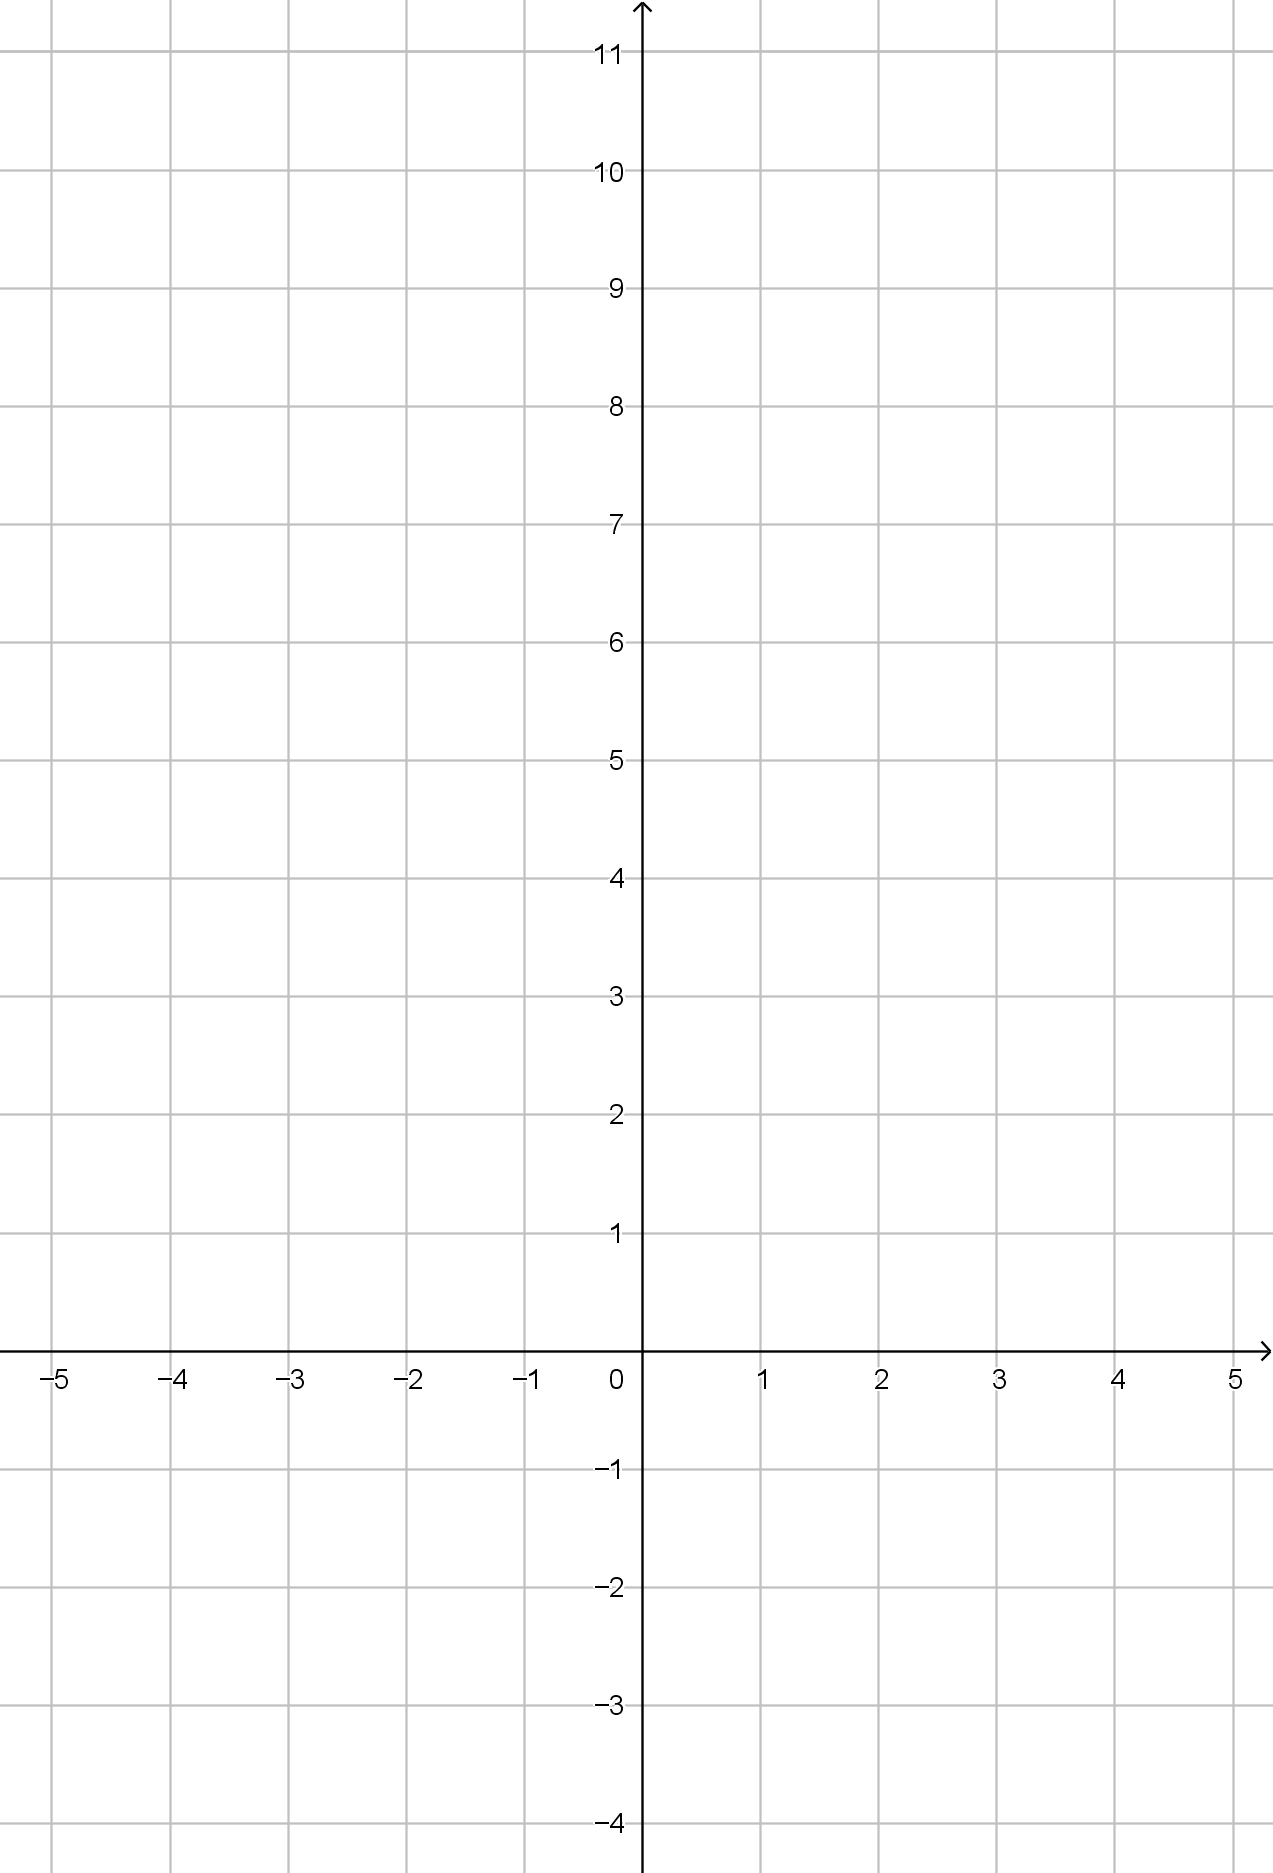
\includegraphics[width=0.4\textwidth]{deri_x^2}}
\begin{enumerate}[(1)]
\item
\(x=1\)에서 \(x=3\) 까지의 평균변화율은 \pb{11}이다.
\item
두 점 \((1,f(1))\), \((3,f(3))\)를 지나는 직선의 방정식은 \(\pb{y=4x-3}\)이다.
\item
\(x=1\)에서 \(x=2\) 까지의 평균변화율은 \pb{11}이다.
\item
두 점 \((1,f(1))\), \((2,f(2))\)를 지나는 직선의 방정식은 \(\pb{y=3x-2}\)이다.
\item
\(x=1\)에서 \(x=x\) 까지의 평균변화율은 \pb{x+1}이다.
\item
\(x=1\)에서의 순간변화율 \(f'(1)\)은 \pb{2}이다.
\item
\(x=1\)에서 \(x=1+h\) 까지의 평균변화율은 \pb{h+2}이다.
\item
\(x=1\)에서의 순간변화율 \(f'(1)\)은 \pb{2}이다.
\item
점 \((1,f(1))\)에서의 접선의 방정식은 \(\pb{y=2x-2}\)이다. 
\end{enumerate}
\newpage

%
\exam{\(f(x)=-x^2+2x+8\)}
{\centering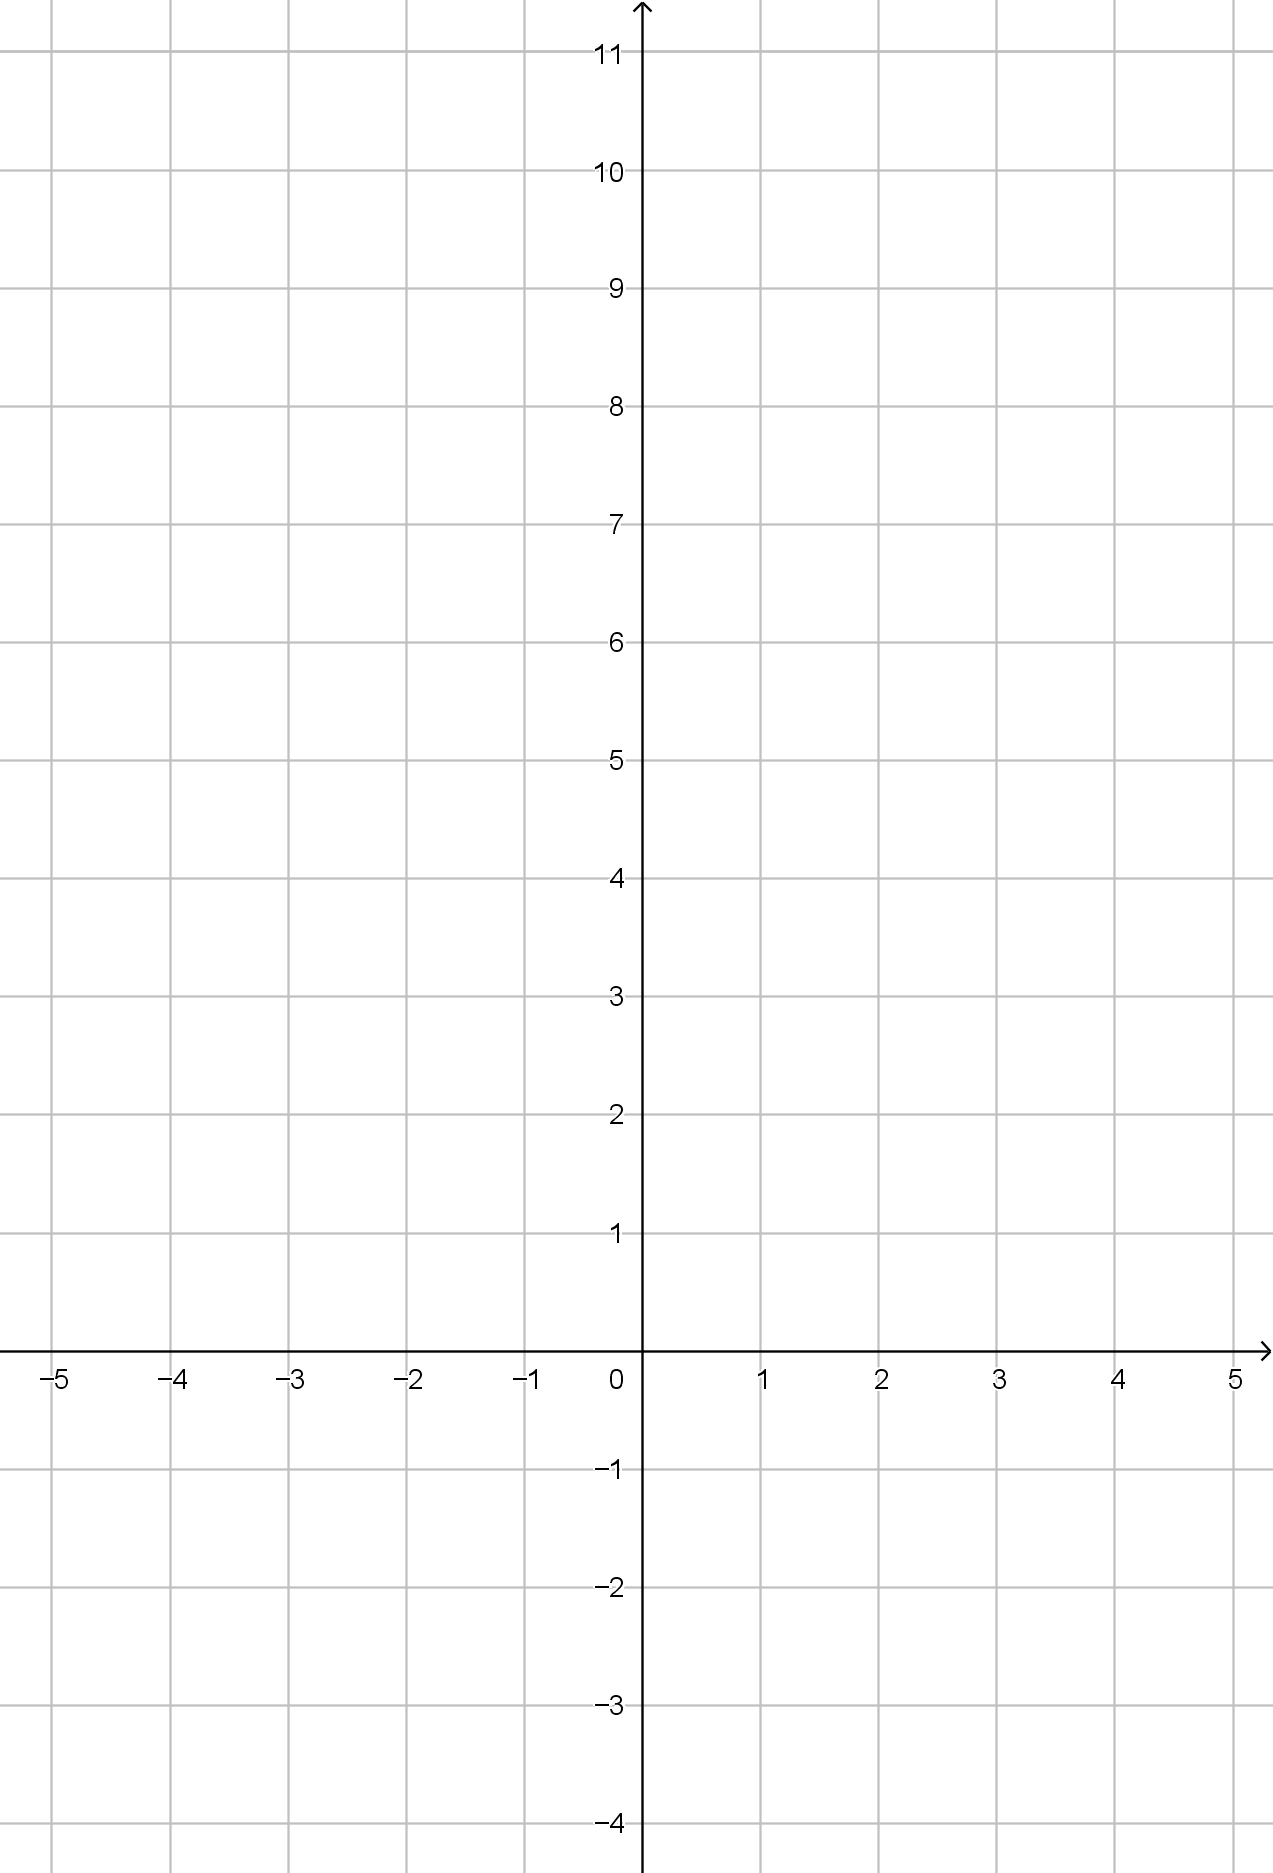
\includegraphics[width=0.4\textwidth]{deri_x^2}}
\begin{enumerate}[(1)]
\item
\(x=2\)에서 \(x=4\) 까지의 평균변화율은 \pb{11}이다.
\item
두 점 \((2,f(2))\), \((4,f(4))\)를 지나는 직선의 방정식은 \(\pb{y=4x-3}\)이다.
\item
\(x=2\)에서 \(x=3\) 까지의 평균변화율은 \pb{11}이다.
\item
두 점 \((2,f(2))\), \((3,f(3))\)를 지나는 직선의 방정식은 \(\pb{y=3x-2}\)이다.
\item
\(x=2\)에서 \(x=x\) 까지의 평균변화율은 \pb{x+1}이다.
\item
\(x=2\)에서의 순간변화율 \(f'(2)\)은 \pb{2}이다.
\item
\(x=2\)에서 \(x=2+h\) 까지의 평균변화율은 \pb{h+2}이다.
\item
\(x=2\)에서의 순간변화율 \(f'(2)\)은 \pb{2}이다.
\item
점 \((2,f(2))\)에서의 접선의 방정식은 \(\pb{y=2x-2}\)이다. 
\end{enumerate}
\newpage

%
\exam{\(f'(2)=3\)일 때, 다음 극한값들을 구하여라.}
\begin{align*}
(1)&\:\:
\lim_{h\to0}\frac{f(2+3h)-f(2)}{h}
=\lim_{h\to0}\frac{f(2+3h)-f(2)}{3h}\times3\\
&=f'(2)\times3=9\\
(2)&\:\:
\lim_{h\to0}\frac{f(2+h)-f(2-h)}{h}\\
&=\lim_{h\to0}\frac{\left\{f(2+h)-f(2)\right\}-\left\{f(2-h)-f(2)\right\}}{h}\\
&=\lim_{h\to0}\frac{f(2+h)-f(2)}h
+\lim_{h\to0}\frac{f(2-h)-f(2)}{-h}\\
&=f'(2)+f'(2)=6\\
(3)&\:\:
\lim_{x\to2}\frac{f(x)-f(2)}{x^2-4}
=\lim_{x\to2}\frac{f(x)-f(2)}{(x-2)(x+2)}\\
&=\lim_{x\to2}\frac{f(x)-f(2)}{x-2}\times\lim_{x\to2}\frac1{x+2}\\
&=f'(2)\times\frac14=\frac34\\
(4)&\:\:
\lim_{x\to2}\frac{x^3-8}{f(x)-f(2)}
=\lim_{x\to2}\frac{(x-2)(x^2+2x+4)}{f(x)-f(2)}\\
&=\lim_{x\to2}\frac{x^2+2x+4}{\frac{f(x)-f(2)}{x-2}}\\
&=\frac{12}{f'(2)}=4
\end{align*}

%
\prob{\(f'(1)=2\)일 때, 다음 극한값들을 구하여라.}
\begin{align*}
(1)\:\:&\lim_{h\to0}\frac{f(1+2h)-f(1)}{h}=\phantom{11111111111111}\\
(2)\:\:&\lim_{h\to0}\frac{f(1+h)-f(1)}{2h}=\\
(3)\:\:&\lim_{h\to0}\frac{f(1+h)-f(1-h)}h=\\
(4)\:\:&\lim_{x\to1}\frac{f(x)-f(1)}{x^3-1}=\\
(5)\:\:&\lim_{x\to1}\frac{x^2-1}{f(x)-f(1)}=\\
(6)\:\:&\lim_{x\to1}\frac{f(x)-f(1)}{\sqrt x-1}=
\end{align*}
\newpage

%
\begin{mdframed}[frametitle=미분가능성]
\(f(x)\)가 \(x=a\)에서 미분가능하다.\\
\(\iff\)\(f'(a)\)가 존재한다.\\[2ex]
\(\displaystyle\iff\pb{\lim_{x\to a}\frac{f(x)-f(a)}{x-a}}\)가 존재한다.\\[2ex]
\(\iff\displaystyle
\pb{\lim_{x\to a-}\frac{f(x)-f(a)}{x-a}}
=
\pb{\lim_{x\to a+}\frac{f(x)-f(a)}{x-a}}\)
\end{mdframed}

%
\begin{mdframed}[frametitle=미분가능성과 연속]
미분가능하면 연속이다.\\
하지만 연속이라고 해서 미분가능한 것은 아니다.
\end{mdframed}

%
\exam{\(f(x)=x^2\)}
{\centering\includegraphics[width=0.4\textwidth]{55}}
\begin{enumerate}[(1)]
\item
\(\displaystyle f(1)=\lim_{x\to1}f(x)\)이 성립한다 / 성립하지 않는다.
\item
\(f(x)\)는 \(x=1\)에서 연속이다 / 연속이 아니다.
\item
\(y=f(x)\)의 그래프는 \(x=1\)에서 이어져있다 / 끊어져있다.
\item
\(f'(1)\)이 존재한다 / 존재하지 않는다.
\item
\(f(x)\)는 \(x=1\)에서 미분가능하다 / 미분불가능하다
\item
\(y=f(x)\)의 그래프는 \(x=1\)에서 접선을 그을 수 있다 / 그을 수 없다.
\end{enumerate}
\newpage

%
\exam{\(f(x)=x|x-2|\)}
{\centering\includegraphics[width=0.4\textwidth]{55}}
\begin{enumerate}[(1)]
\item
\(\displaystyle f(2)=\lim_{x\to2}f(x)\)이 성립한다 / 성립하지 않는다.
\item
\(f(x)\)는 \(x=2\)에서 연속이다 / 연속이 아니다.
\item
\(y=f(x)\)의 그래프는 \(x=2\)에서 이어져있다 / 끊어져있다.
\item
\(f'(2)\)이 존재한다 / 존재하지 않는다.
\item
\(f(x)\)는 \(x=2\)에서 미분가능하다 / 미분불가능하다
\item
\(y=f(x)\)의 그래프는 \(x=2\)에서 접선을 그을 수 있다 / 그을 수 없다.
\end{enumerate}
\newpage

%
\exam{\(f(x)=|x-1|\)}
{\centering\includegraphics[width=0.4\textwidth]{55}}
\begin{enumerate}[(1)]
\item
\(\displaystyle f(1)=\lim_{x\to1}f(x)\)이 성립한다 / 성립하지 않는다.
\item
\(f(x)\)는 \(x=1\)에서 연속이다 / 연속이 아니다.
\item
\(y=f(x)\)의 그래프는 \(x=1\)에서 이어져있다 / 끊어져있다.
\item
\(f'(1)\)이 존재한다 / 존재하지 않는다.
\item
\(f(x)\)는 \(x=1\)에서 미분가능하다 / 미분불가능하다
\item
\(y=f(x)\)의 그래프는 \(x=1\)에서 접선을 그을 수 있다 / 그을 수 없다.
\end{enumerate}
\newpage

%
\exam{\(f(x)=\frac{x^3-x^2-6x}{x-3}\)}
{\centering\includegraphics[width=0.4\textwidth]{55}}
\begin{enumerate}[(1)]
\item
\(\displaystyle f(3)=\lim_{x\to3}f(x)\)이 성립한다 / 성립하지 않는다.
\item
\(f(x)\)는 \(x=3\)에서 연속이다 / 연속이 아니다.
\item
\(y=f(x)\)의 그래프는 \(x=3\)에서 이어져있다 / 끊어져있다.
\item
\(f'(3)\)이 존재한다 / 존재하지 않는다.
\item
\(f(x)\)는 \(x=3\)에서 미분가능하다 / 미분불가능하다
\item
\(y=f(x)\)의 그래프는 \(x=3\)에서 접선을 그을 수 있다 / 그을 수 없다.
\end{enumerate}
\newpage

\end{document}